\documentclass[11pt,a4paper]{article}
\usepackage[margin=22mm,headheight=16pt,footskip=12mm]{geometry}
\usepackage[T1]{fontenc}
\usepackage[utf8]{inputenc}
\usepackage{lmodern,amsmath,amssymb,graphicx,xcolor,booktabs,longtable,array,tabularx}
\usepackage{tikz,float,caption,fancyhdr,titlesec,url,lscape}
\usetikzlibrary{arrows.meta,positioning,calc}
\definecolor{navy}{HTML}{16324F}
\definecolor{teal}{HTML}{007F86}
\definecolor{pale}{HTML}{EAF5F5}
\definecolor{ink}{HTML}{243646}
\definecolor{amber}{HTML}{A45C13}
\pdfinfo{/Title (Inverse-GPR Virtual-Fuel PI Controller) /Author (T-MATS Controller Development Study)}
\urlstyle{tt}
\setlength{\parindent}{0pt}
\setlength{\parskip}{5pt plus 1pt minus 1pt}
\setlength{\emergencystretch}{2em}
\widowpenalty=10000\clubpenalty=10000
\linespread{1.05}
\titleformat{\section}{\Large\sffamily\bfseries\color{navy}}{\thesection}{.7em}{}
\titleformat{\subsection}{\large\sffamily\bfseries\color{teal}}{\thesubsection}{.7em}{}
\titlespacing*{\section}{0pt}{19pt}{8pt}
\titlespacing*{\subsection}{0pt}{13pt}{5pt}
\captionsetup{font=small,labelfont={bf,color=navy},skip=8pt}
\pagestyle{fancy}\fancyhf{}
\fancyhead[L]{\small\sffamily\color{navy}INVERSE GPR: THREE REMEDIES}
\fancyhead[R]{\small\sffamily T-MATS control study}
\fancyfoot[L]{\scriptsize\color{ink}Three remedies / measured feedback tradeoffs}
\fancyfoot[R]{\small\thepage}
\renewcommand{\headrulewidth}{.3pt}
\tikzset{block/.style={draw=navy!55,fill=navy!3,rounded corners=3pt,minimum height=.92cm,align=center,font=\sffamily\small,inner sep=5pt},
gp/.style={block,draw=teal,fill=pale},plant/.style={block,draw=navy,fill=navy!12},
sum/.style={circle,draw=navy,minimum size=.68cm,fill=white,font=\large},
arr/.style={-{Latex[length=2.2mm]},draw=navy,line width=.65pt},
lab/.style={font=\small,fill=white,inner sep=2pt},
note/.style={font=\small\sffamily,text=ink,align=left}}
\begin{document}
\begin{titlepage}\color{navy}\sffamily
{\small T-MATS / INVERSE GPR / CONTROLLER REDESIGN}\par\vspace{20mm}
{\fontsize{29}{35}\selectfont\bfseries Why the Inverse PI Rang\\and Three Implemented\\Remedies\par}
\vspace{10mm}{\Large Diagnosis, joint-objective tuning,\\and frozen-parameter environmental transfer\par}
\vspace{10mm}\color{teal}\rule{\linewidth}{1.2pt}\color{navy}\vspace{10mm}
\begin{tabular}{@{}ll}
Target & 4000 m, ISA+5, 9500 rpm, 10\% shaft-load steps\\[5pt]
GPR & Same frozen four-input exact posterior\\[5pt]
R1 & Retuned original inverse PI\\[5pt]
R2 & Split static-error integration / weighted acceleration feedback\\[5pt]
R3 & Slope-normalized inverse feedback with a guarded fallback\\[5pt]
Evaluation & 80 tuning candidates; 105 grid-transfer runs
\end{tabular}
\par\vspace{12mm}\normalfont\color{ink}
The expectation that a more accurate inverse must improve both speed error and fuel ringing does not hold automatically. Regression accuracy concerns the predicted fuel values; closed-loop behaviour also depends on inverse derivatives, delay, feedback structure and controller gains. This study identifies those mechanisms, implements three alternatives and measures their tradeoffs against both base PI and the previous inverse controller.

\vfill All changes are simulated. The inherited compressor-map limits remain in force; numerical convergence outside those limits is not physical engine validation.
\end{titlepage}
\tableofcontents\clearpage

\section{Why the earlier expectation was not met}
The prior environmental inverse GP achieved about 0.00161 lbm/s RMSE on 200 held-out samples, yet the controller at 4000 m/ISA+5 produced 1.819 rpm speed RMSE and 3.817 lbm/s fuel ringing. Base PI produced 2.531 rpm and 2.030 lbm/s. The inverse improved the speed metric while making the fuel command substantially more oscillatory. The following mechanisms explain why those results can coexist.

\subsection{The inverse PI contains implicit derivative action}
Write the inverse as $v=g(N,a,T,P)$. At a fixed environment and near the reference,
\begin{equation}
e_v=g(r,0,T,P)-g(N,\hat a,T,P)\simeq g_N e_N+g_a\dot e_N.
\end{equation}
Applying a PI to this virtual error yields, in an ideal local interpretation,
\begin{equation}
\left(K_p+\frac{K_i}{s}\right)(g_N+g_as)
=K_pg_as+(K_pg_N+K_ig_a)+\frac{K_ig_N}{s}.
\end{equation}
Acceleration therefore enters the proportional \emph{and integral} paths. With the previous gains, the target's effective proportional coefficient is approximately 0.0503, about twice the base PI value 0.025, while the implicit derivative coefficient is 0.00316. Keeping numerical gains after retraining the GP did not preserve feedback bandwidth or damping.

\begin{table}[H]\centering\small\setlength{\tabcolsep}{5pt}
\begin{tabular}{@{}lrrrrr@{}}\toprule
m/ISA & $g_N$ & $g_a$ & $K_{P,eq}$ & $K_{I,eq}$ & $g_a/g_N$ (s)\\\midrule
4000/+5 & 0.00145757 & 0.00157863 & 0.050274 & 0.043727 & 1.0831\\
5000/-30 & -6.52288e-05 & 0.00150339 & 0.044971 & -0.0019569 & -23.048\\
\bottomrule\end{tabular}\caption{Verified derivatives of the unchanged GP at 9500 rpm and zero acceleration. The previous gains are Kp=2, Ki=30.}\end{table}

The analytical GP derivatives were checked against independent central finite differences; the largest absolute discrepancy over the grid and target is 1.72e-09. At the target, the relation $e_v\simeq0$ leaves a speed-error tail with local time constant $g_a/g_N\simeq1.083$ s. Small virtual error therefore does not imply fast elimination of speed error.

\subsection{Filtering, training inputs and feedforward matter}
The identification labels used true plant acceleration, whereas online feedback uses a filtered derivative of a sensed speed. Sensor lag and acceleration filtering alter the effective inverse feedback. The prior target run briefly left the training acceleration range. There was no added sensor noise in these simulations: the ringing cannot be blamed on injected noise. Derivative-like feedback and phase lag can produce oscillatory fuel commands even with deterministic signals. Derivative filtering is a standard bandwidth/noise tradeoff~\cite{pid}; increasing filtering alone also adds lag.

The feedforward term is constant at constant speed reference and constant inlet state. A residual integral absorbs that constant offset. It cannot anticipate an unknown shaft-load step, so it offers no inherent disturbance-rejection advantage in this particular test.

\subsection{Value accuracy did not constrain inverse slopes}
9 environments have a negative learned static speed slope at the nominal setpoint. At 5000 m/ISA-30, $g_N\simeq-6.52\times10^{-5}$ reverses the previous controller's effective integral action. The observed late speed drift is consistent with this local feedback defect. These conditions also involve the original compressor-map boundary behaviour. Low value-prediction RMSE is not a guarantee of useful derivative signs, and GP response standard deviation is not a certificate of feedback stability.

\section{Three implemented solutions}
All three retain the same four-input exact GPR, plant, fuel limits, 0.015 s sampling, speed sensor, startup preparation and disturbance definition. The GP is not retrained. The changes below isolate feedback structure and tuning.

\subsection{R1: retune the existing inverse PI}
R1 preserves the original equations:
\begin{align}
e_v&=g(r,0,T,P)-g(N_s,\hat a_s,T,P),\\
u^*&=g(r,0,T,P)+K_pe_v+I,\qquad \dot I=K_i e_v.
\end{align}
Gains are selected using both speed RMSE and fuel ringing. This is the least disruptive remedy. It can reduce the excessive feedback action, but it retains the inverse-induced settling tail and cannot correct a negative static inverse slope. Very low gains removed most ringing in initial trials but produced unacceptable tracking tradeoffs; those trials remain in the tuning record.

\subsection{R2: split integration from acceleration feedback}
Define a static inverse error and a separate acceleration contribution:
\begin{align}
e_0&=g(r,0,T,P)-g(N_s,0,T,P),\\
\Delta v_a&=g(N_s,\hat a_s,T,P)-g(N_s,0,T,P),\\
u^*&=g(r,0,T,P)+K_p(e_0-\beta\Delta v_a)+I,\qquad \dot I=K_i e_0.
\end{align}
Only the static error is integrated. The weight $\beta$ independently limits acceleration feedback instead of tying its entire effect to the static proportional gain. Locally,
\begin{equation}
K_{P,eq}=K_pg_N,\qquad K_{I,eq}=K_ig_N,\qquad K_{D,eq}=\beta K_pg_a.
\end{equation}
The unwanted $K_i g_a$ proportional contribution is removed, and integral action enforces static speed agreement rather than the dynamic virtual-error condition. Simply removing the acceleration integral without restoring appropriate static damping performed poorly in the initial trials. R2 was therefore tuned with separate acceleration attenuation. A negative $g_N$ remains a limitation because R2 retains the static inverse error sign.

\subsection{R3: normalize inverse slopes and separate damping}
Evaluate setpoint derivatives $g_N,g_a$ from the frozen posterior and form
\begin{equation}
\tilde e_N=\frac{g(r,0,T,P)-g(N_s,0,T,P)}{g_N},\qquad
\tilde a=\frac{g(N_s,\hat a_s,T,P)-g(N_s,0,T,P)}{g_a}.
\end{equation}
R3 controls in approximate speed-domain units:
\begin{equation}
u^*=g(r,0,T,P)+K_p\tilde e_N-K_d\tilde a+I,\qquad \dot I=K_i\tilde e_N.
\end{equation}
This allows direct selection of speed-error proportional/integral action and acceleration damping rather than allowing GP slopes to set all three implicitly. It is not the original virtual-fuel PI with a new label.

Normalization is guarded. If either derivative is at most $10^{-5}$ in its corresponding physical units, the monitored compressor corrected speed is outside $[0.5,1.05]$, or $\tilde e_N/e_N$ lies outside $[0.25,4]$ for $|e_N|>0.01$ rpm, the feedback substitutes $\tilde e_N=e_N$ and $\tilde a=\hat a_s$. The GP feedforward remains present. This is an explicit hybrid inverse/speed-feedback controller; its fallback prevents unreliable inverse error polarity from determining feedback. It does not extend the physical compressor map.

All implementations use conditional integration at the shared fuel limits and track the startup PI before the 45 s handover. The acceleration estimate remains causal:
\begin{equation}
\hat a_s[k]=p_a\hat a_s[k-1]+(1-p_a)\frac{N_s[k]-N_s[k-1]}{T_s},\qquad p_a=e^{-T_s/\tau_a}.
\end{equation}

\section{Tuning objective, selection and parameters}
The target case is now explicitly a tuning case. It must not be described as independent validation of the selected gains. Candidates were explored in an initial grid, followed by refinements where the first grid exposed slow recovery or insufficient static damping. All 80 trials are retained.

For each accepted candidate, define
\begin{equation}
J=\max\left(\frac{\mathrm{RMSE}}{\mathrm{RMSE}_{\rm base}},\frac{R}{R_{\rm base}}\right).
\end{equation}
The minimum $J$ in each family is selected. A value below one improves both metrics relative to base PI. This balanced objective does not necessarily select the smallest speed RMSE or smallest ringing alone, and it does not guarantee improvement over the previous inverse controller's already lower speed RMSE.

\begin{table}[H]\centering\small\setlength{\tabcolsep}{5pt}
\begin{tabular}{@{}lrrrrr@{}}\toprule
Remedy & $K_p$ & $K_i$ & $K_d$ & $\tau_a$ (s) & $\beta$\\\midrule
R1 & 1.5 & 22 & 0 & 0.03 & 1\\
R2 & 16 & 40 & 0 & 0.03 & 0.05\\
R3 & 0.025 & 0.1 & 0.002 & 0.03 & 1\\
\bottomrule\end{tabular}\caption{Selected parameters. R1/R2 gains act on virtual fuel; R3 gains act on normalized speed/acceleration. Kd is used only by R3, beta only by R2. Their numerical gains are not directly comparable across architectures.}\end{table}

\begin{table}[H]\centering\small\setlength{\tabcolsep}{5pt}
\begin{tabular}{@{}rrrrrl@{}}\toprule
Candidate & Remedy & RMSE/base & Ring/base & Joint score & Both lower\\\midrule
48 & 1 & 0.963 & 0.886 & 0.963 & yes\\
64 & 2 & 0.918 & 0.338 & 0.918 & yes\\
78 & 3 & 0.692 & 0.719 & 0.719 & yes\\
\bottomrule\end{tabular}\caption{Winner of each remedy family under the declared joint score. These target-case results are tuning results, not independent hold-out validation.}\end{table}

These parameters are frozen before the 35-condition grid evaluation. The earlier base-PI and inverse-controller trajectories are reused as deterministic comparators with identical plant configuration, initial preparation and condition-specific load amplitudes. Three selected target trajectories come from the tuning records; 105 new simulations apply the three fixed selections over the environmental grid.

\begin{figure}[H]\centering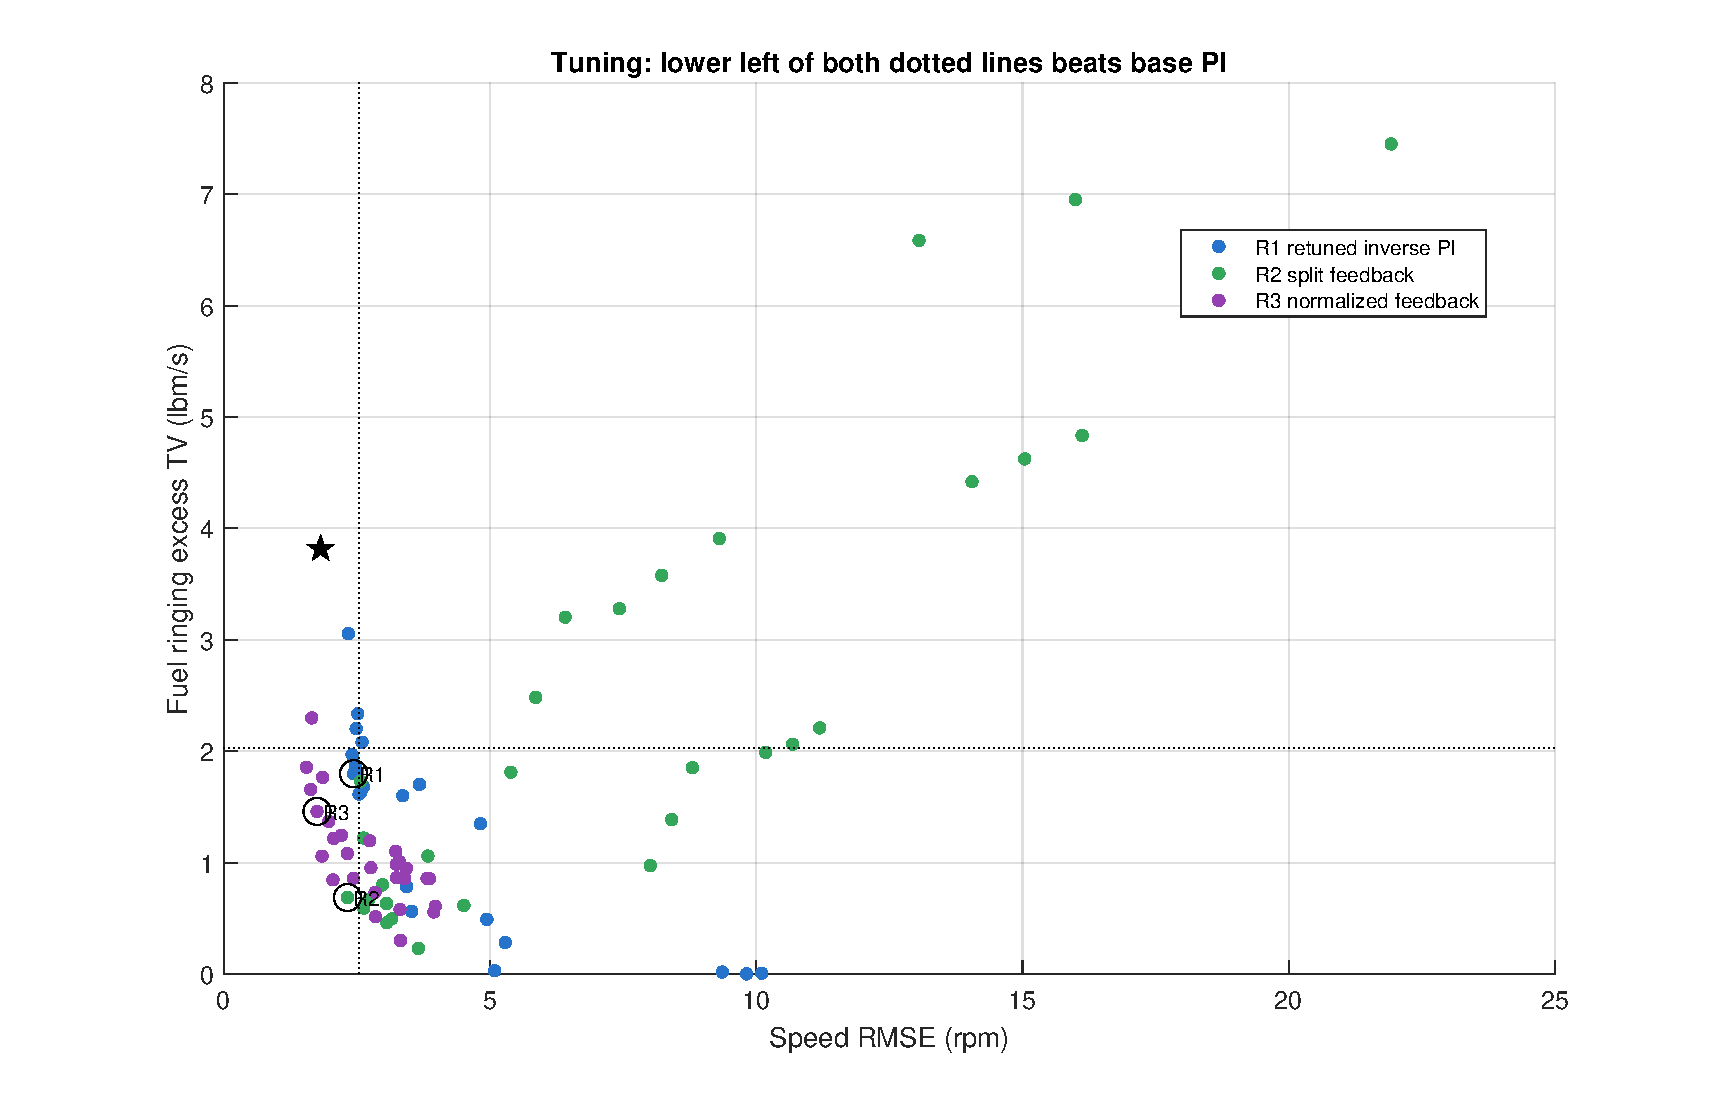
\includegraphics[width=\linewidth]{remedy_tuning.pdf}\caption{All accepted tuning candidates. Dotted lines mark base-PI performance, black circles mark selected remedies, and the black star marks the previous inverse PI.}\end{figure}


\section{Measured target-case comparison}
\begin{table}[H]\centering\small\setlength{\tabcolsep}{5pt}
\begin{tabular}{@{}lrrrrrr@{}}\toprule
Method & RMSE & Ringing & Peak error & $t_{1\%}$ & $t_{0.1}$ & Min. SM\\\midrule
Base PI & 2.531 & 2.03 & 21.59 & 0 & 2.46 & 9.01\\
Previous inverse & 1.819 & 3.817 & 13.4 & 0 & NR & 8.73\\
R1 & 2.439 & 1.798 & 15.34 & 0 & NR & 9.81\\
R2 & 2.323 & 0.6861 & 16.77 & 0 & 1.53 & 10.8\\
R3 & 1.752 & 1.459 & 14.39 & 0 & 1.38 & 10.4\\
\bottomrule\end{tabular}\caption{4000 m/ISA+5, 9500 rpm, 10\% shaft-load steps. RMSE and peak error: rpm; ringing: lbm/s; recovery: s; surge margin: percent. NR means no persistent recovery before the next edge or evaluation end.}\end{table}

R1: RMSE changes by -3.7\% and ringing by -11.4\% relative to base PI. Relative to the previous inverse controller, the changes are +34.1\% and -52.9\%, respectively.

R2: RMSE changes by -8.2\% and ringing by -66.2\% relative to base PI. Relative to the previous inverse controller, the changes are +27.7\% and -82.0\%, respectively.

R3: RMSE changes by -30.8\% and ringing by -28.1\% relative to base PI. Relative to the previous inverse controller, the changes are -3.7\% and -61.8\%, respectively.

\begin{table}[H]\centering\small\setlength{\tabcolsep}{5pt}
\begin{tabular}{@{}lrrrrr@{}}\toprule
Method & IAE & Peak fuel & Peak slew & GP outside & Fallback\\\midrule
Base PI & 53.5 & 2.13 & 4.67 & 0 & --\\
Previous inverse & 61.3 & 2.15 & 10.6 & 0.5 & --\\
R1 & 83.6 & 2.09 & 8.11 & 0.65 & 0\\
R2 & 45.9 & 2.02 & 6.54 & 0.75 & 0\\
R3 & 30.3 & 2.05 & 8.35 & 0.65 & 0\\
\bottomrule\end{tabular}\caption{Complementary target metrics: IAE rpm s; peak fuel lbm/s; peak event-window slew lbm/s squared; GP input-range excursions and fallback usage percent. A dash denotes an unavailable/not-applicable diagnostic.}\end{table}

R1 illustrates why even two favorable headline metrics are not sufficient: its long settling tail increases integral absolute speed error relative to base PI. R2 and R3 recover to the tight speed band more quickly. R3 improves RMSE and ringing relative to the previous inverse controller, although its peak absolute speed deviation is slightly larger. These distinctions are retained rather than claiming that one design dominates every performance measure.

The 1\% band is $\pm95$ rpm around the setpoint. Zero recovery time means that the response never leaves that broad band, not that the load step has no effect. The supplementary 0.1 rpm criterion exposes fine settling. Recovery requires staying within the band until the next load edge; a short loaded interval can therefore receive NR despite eventual recovery after unloading.

The ringing metric remains the sum, over six two-second edge windows, of fuel total variation minus net fuel change. It measures reversals in lbm/s, not total fuel consumption. Full-run speed RMSE is measured over the same 90 s evaluation interval. The unchanged validity tests require finite signals, positive fuel and surge margin, converged flow residuals, iterations below 200 and a settled pre-test speed.

\subsection{Does the GPR itself explain the improvement?}
\begin{table}[H]\centering\small\setlength{\tabcolsep}{5pt}
\begin{tabular}{@{}lrrr@{}}\toprule
Feedback & RMSE (rpm) & Ringing (lbm/s) & $t_{0.1}$ (s)\\\midrule
R3 normalized GPR & 1.752 & 1.459 & 1.38\\
Matched-gain filtered PID & 1.7491 & 1.4292 & 1.38\\
\bottomrule\end{tabular}\caption{Diagnostic ablation at the target: identical gains, filtering, feedforward, startup and load, with raw sensed speed error and acceleration replacing the normalized inverse signals.}\end{table}

The matched-gain diagnostic forces R3 to use ordinary sensed speed error and filtered acceleration for the entire run. Its near-identical, slightly better results show that the target improvement comes predominantly from feedback structure and tuning, rather than a demonstrated nonlinear-GPR advantage. Near the setpoint, slope normalization makes the inverse signals approximate speed error and acceleration, so this agreement is expected. The frozen GP remains useful as an inverse representation and feedforward source, but this constant-reference disturbance test does not establish superiority over a comparably tuned conventional filtered PID. The ablation is a diagnostic, not a fourth tuned remedy or a grid-wide comparison.

\clearpage
\subsection{Full response}
\begin{figure}[H]\centering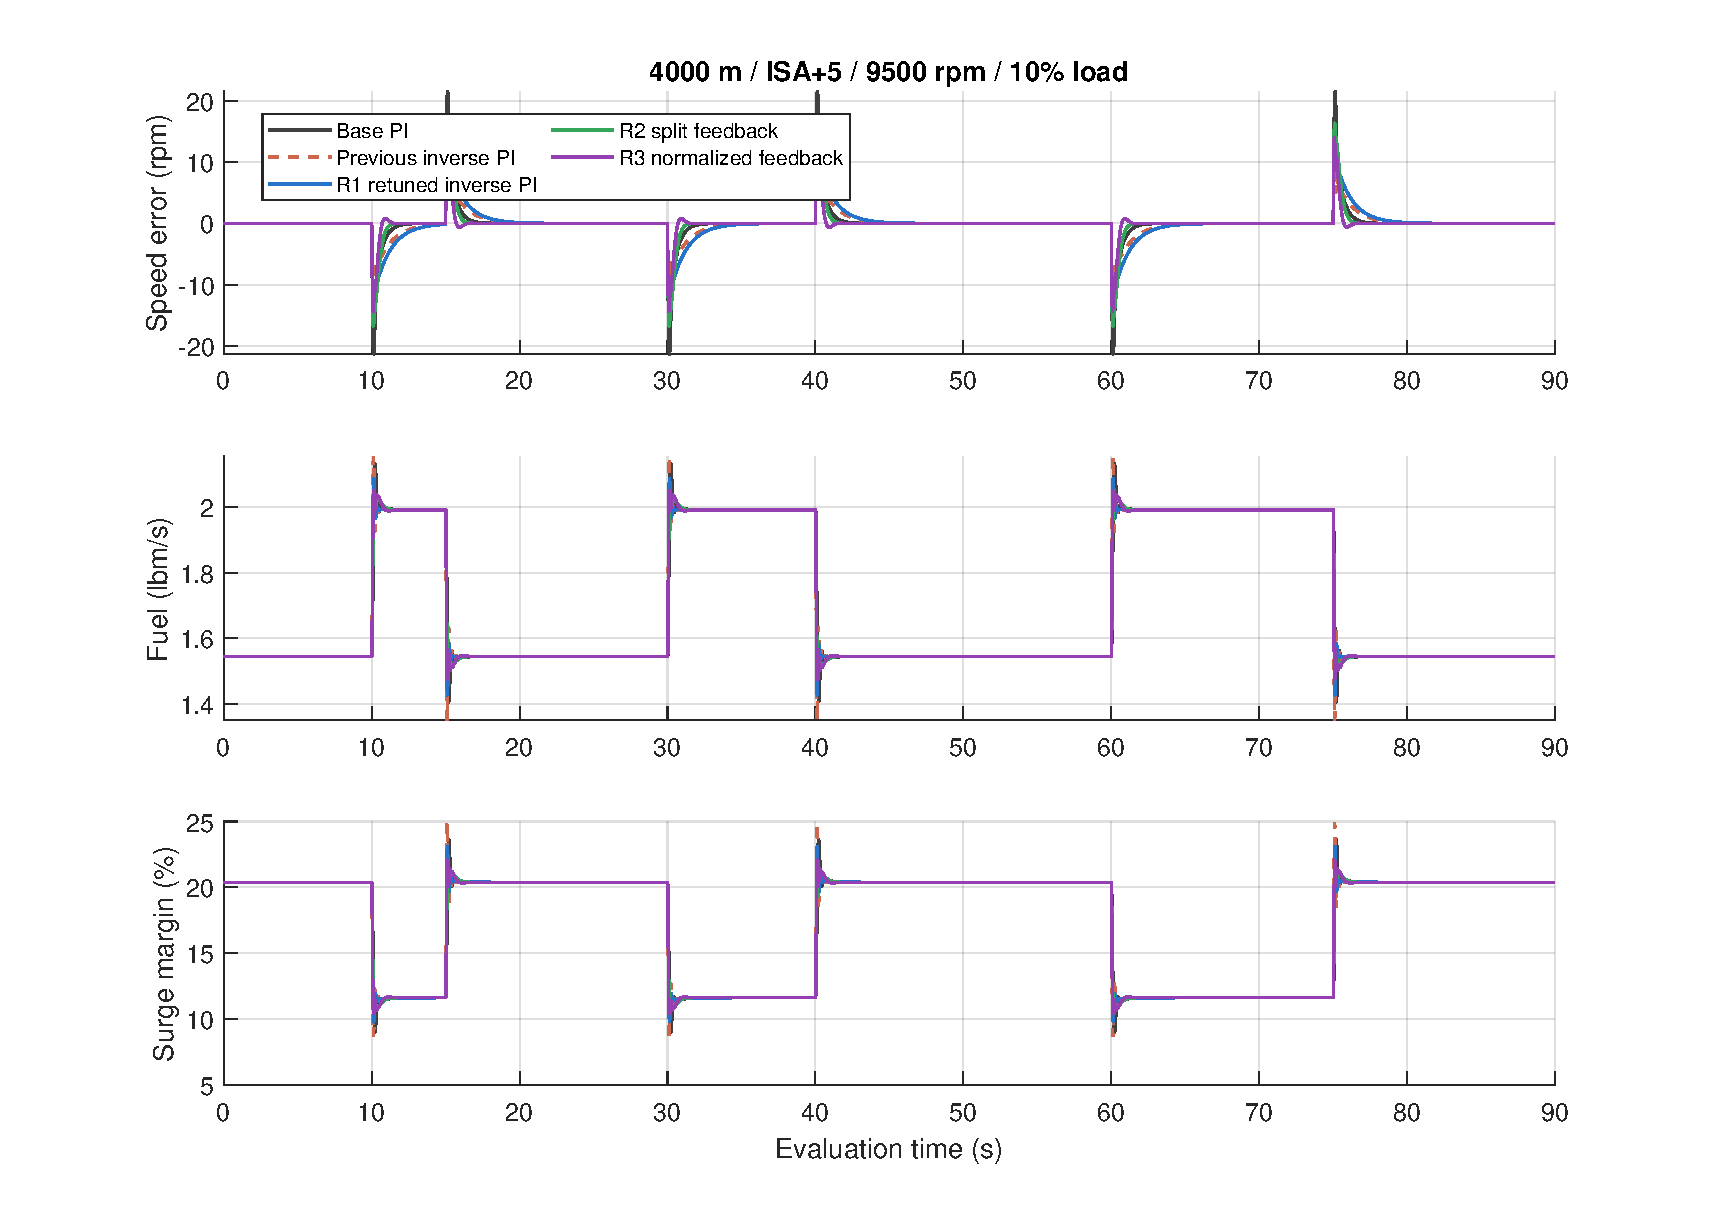
\includegraphics[width=\linewidth]{remedy_overview.pdf}\caption{Full target evaluation with identical load timing and amplitude. The previous inverse controller is retained as an explicit comparator.}\end{figure}

The overview includes the earlier inverse controller so a reduction in fuel ringing is not mistaken for a simultaneous improvement in every tracking metric. All methods see the same three shaft-power pulses; none receives their future schedule.

\clearpage
\subsection{Load application zoom}
\begin{figure}[H]\centering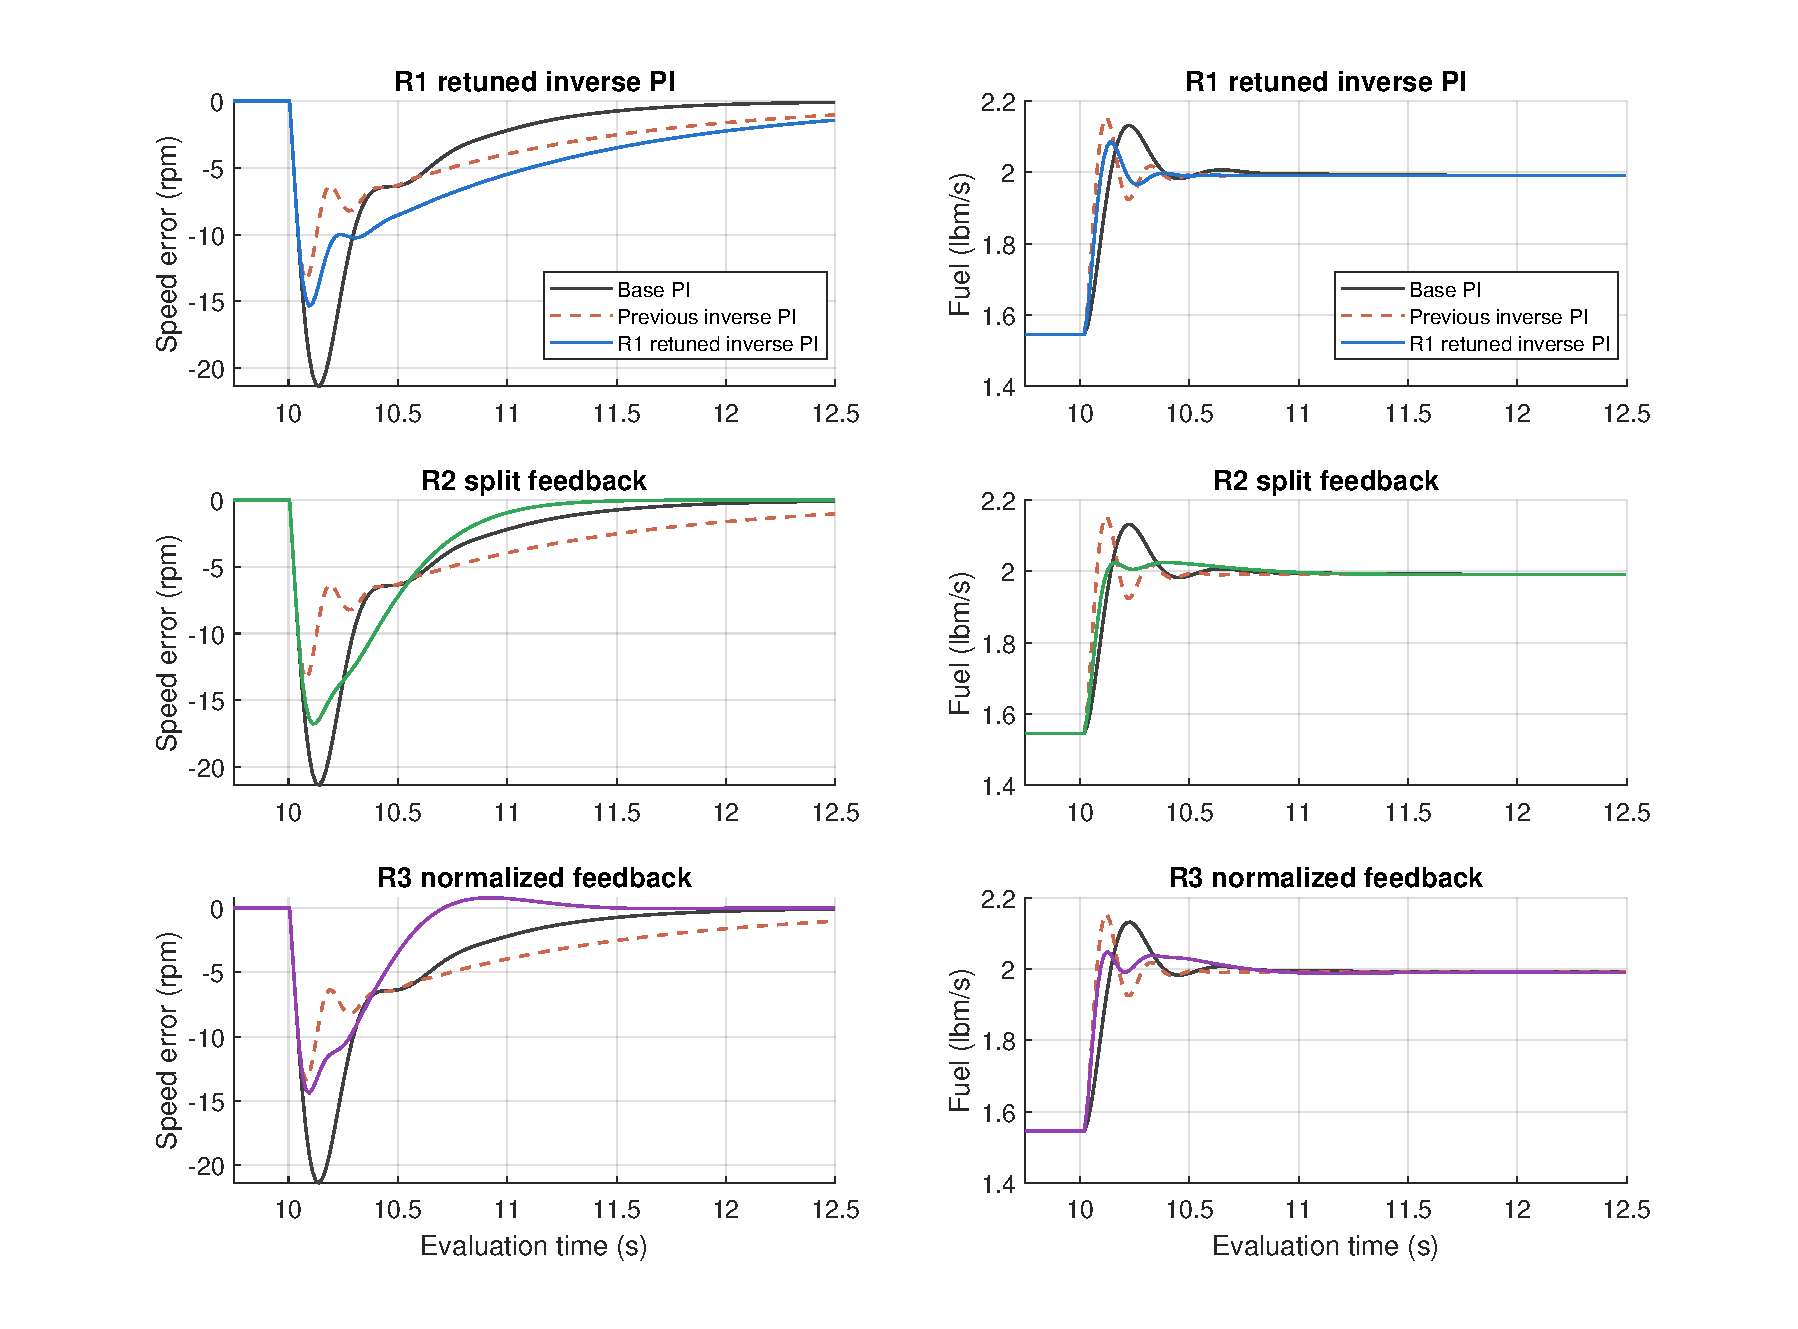
\includegraphics[width=\linewidth]{remedy_load_zoom.pdf}\caption{Detailed first load application: each remedy is compared with base PI and the previous inverse controller.}\end{figure}

The zoom separates the initial speed dip from subsequent fuel reversals. R1 changes the gain balance of the original architecture. R2 changes which error is integrated and attenuates acceleration feedback. R3 removes most operating-point slope scaling from the feedback gain interpretation and retains a separately tuned damping path.

\clearpage
\subsection{Load removal zoom}
\begin{figure}[H]\centering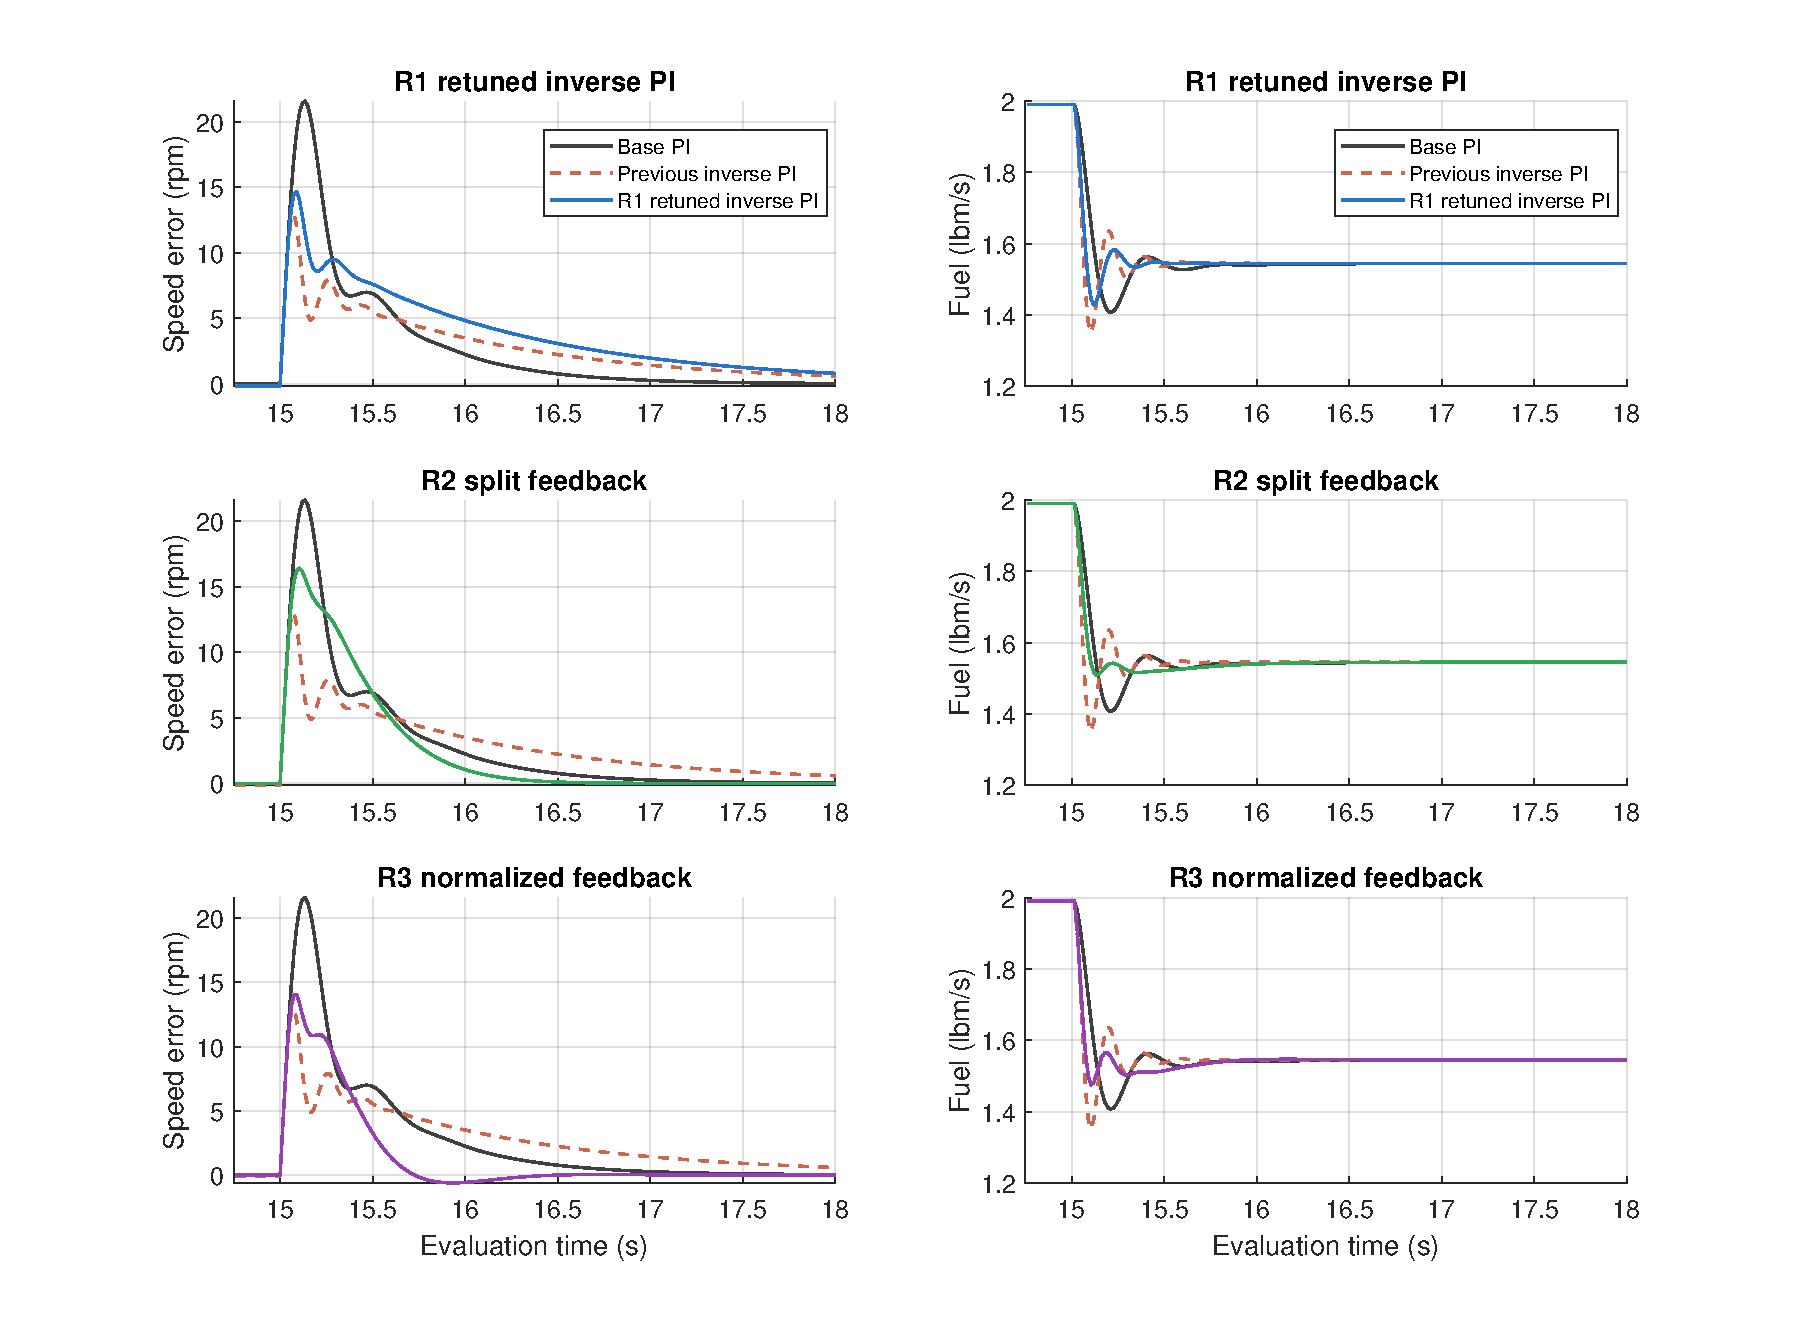
\includegraphics[width=\linewidth]{remedy_unload_zoom.pdf}\caption{Detailed first unloading event. Smoother application alone is insufficient; unloading is also included in the ringing score.}\end{figure}

Load removal provides a complementary test of fuel reduction and overspeed recovery. The score includes both directions; an improvement on application alone is insufficient. The displayed figures use recorded fuel and shaft speed, not a surrogate prediction of the closed-loop response.

\clearpage
\section{Frozen transfer across the environmental grid}
\begin{table}[H]\centering\small\setlength{\tabcolsep}{5pt}
\begin{tabular}{@{}lrrrrrr@{}}\toprule
Method & Accepted & RMSE wins & Ring wins & Both & Both/in map & No 1\% exit\\\midrule
Previous inverse & 35 & 18 & 0 & 0 & 0 & 34\\
R1 & 35 & 9 & 33 & 7 & 7 & 33\\
R2 & 27 & 11 & 25 & 9 & 9 & 25\\
R3 & 35 & 35 & 35 & 35 & 25 & 35\\
\bottomrule\end{tabular}\caption{Counts out of 35 grid conditions. All wins compare paired accepted cases with base PI. Both/in map additionally excludes the monitored compressor corrected-speed overruns. No 1\% exit counts trajectories staying inside the band throughout all six event windows.}\end{table}

Rejected grid cases: R2 at 10000 m/ISA+0; R2 at 10000 m/ISA-10; R2 at 10000 m/ISA+10; R2 at 5000 m/ISA-20; R2 at 7500 m/ISA-20; R2 at 10000 m/ISA-20; R2 at 7500 m/ISA-30; R2 at 10000 m/ISA-30. These cases receive no performance score. R3 used its speed-feedback fallback in 10 of the 35 environments. R3 improves both metrics in all 35 cases, including all 25 cases without a monitored compressor-map speed overrun. R1 improves both in 7 cases and R2 in 9; eight R2 cases are rejected. The most broadly supported choice is R3; R2 is the smoothest target-case option but its target tuning does not establish reliable grid-wide transfer. R1 is a minimal modification with a remaining slow-tail and slope-sign limitation.
The grid retains the five altitudes and seven ISA departures from the environmental study. Training of the GP already included these environments; this is a fixed-controller transfer check under shaft-load disturbances, not an unseen-environment GP validation. The 4000 m/ISA+5 condition is the gain-tuning condition in the present study.

\begin{figure}[H]\centering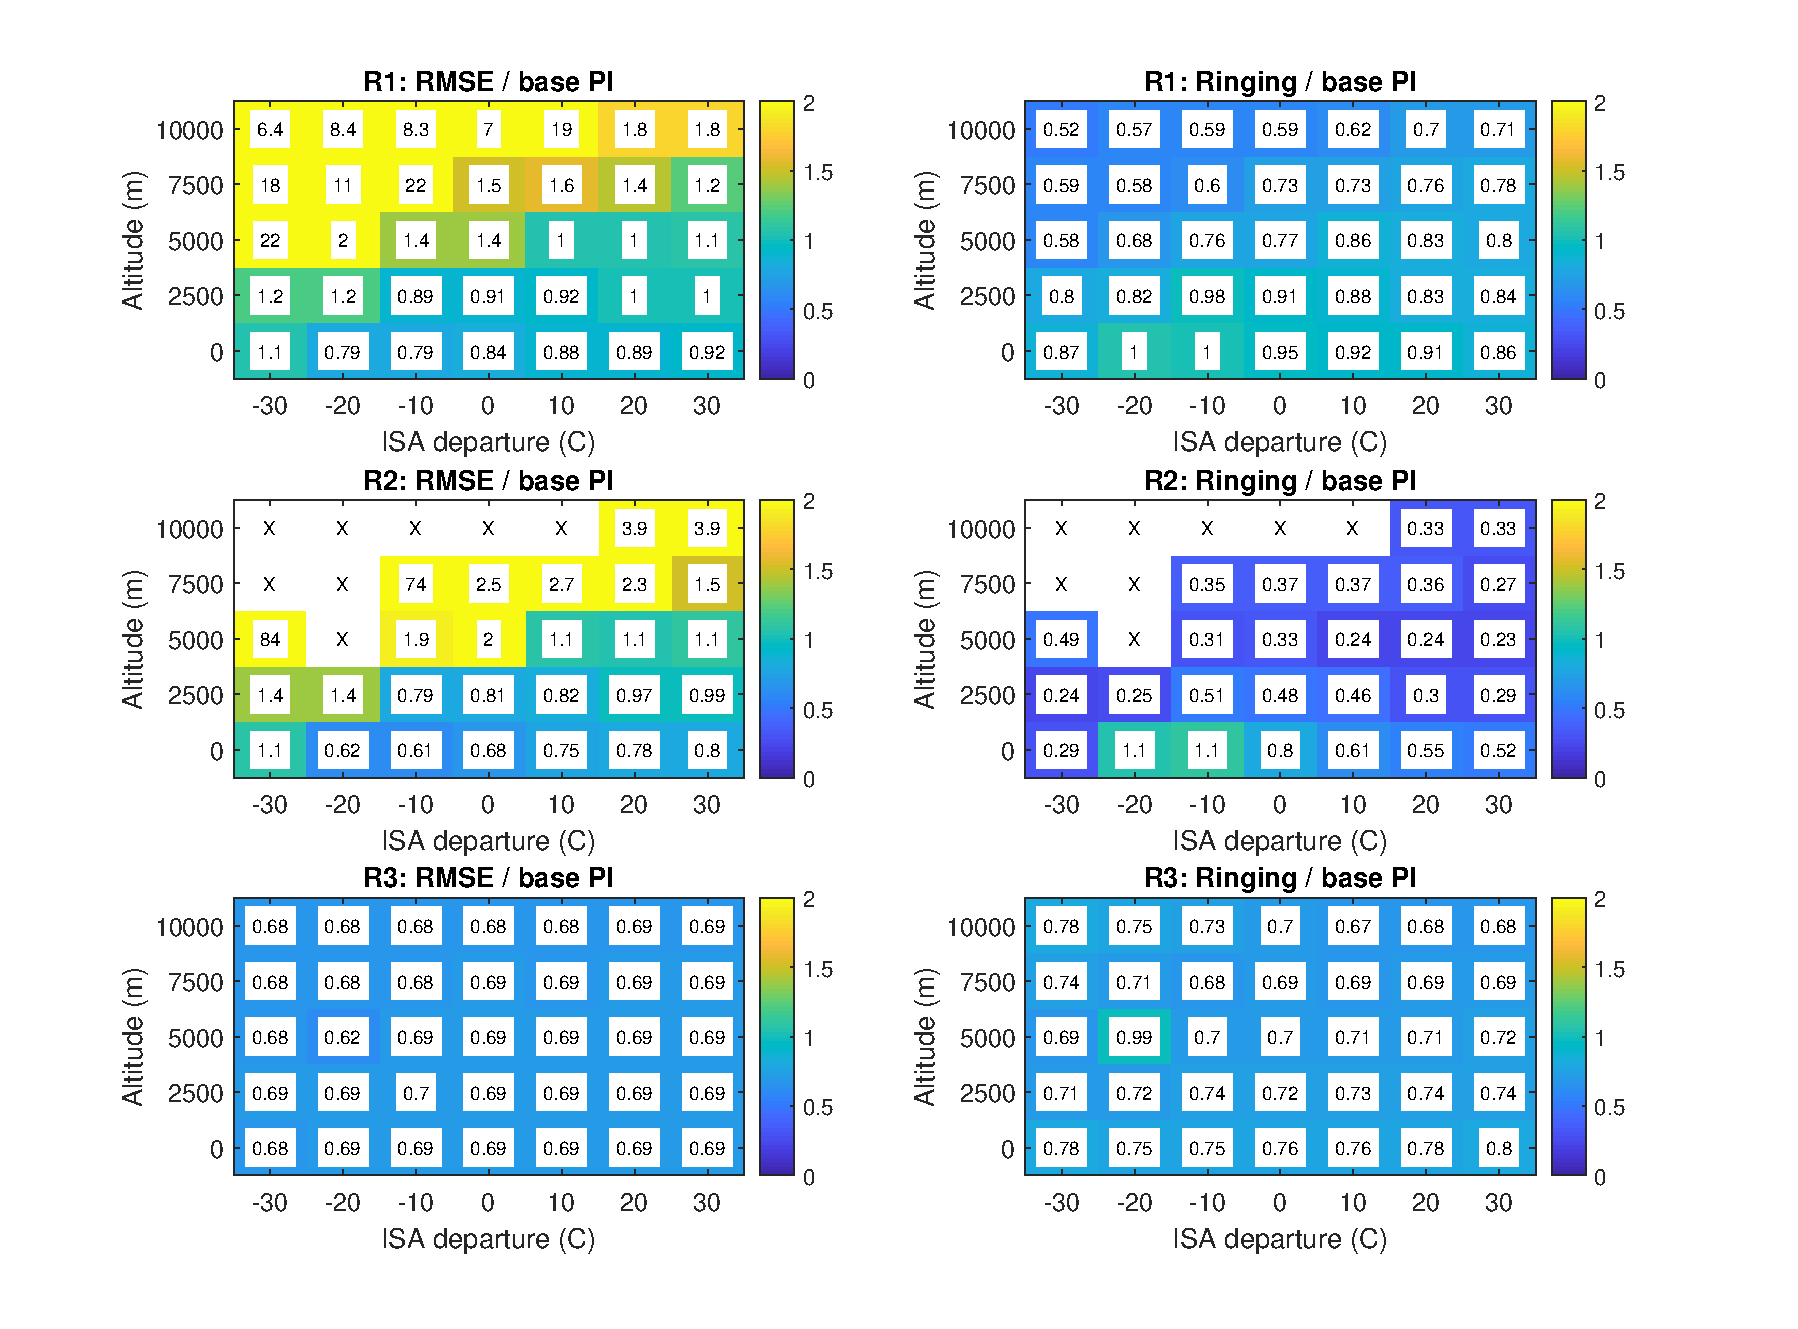
\includegraphics[width=\linewidth]{remedy_grid_ratios.pdf}\caption{Frozen-parameter transfer. Ratios below one improve on base PI; colour is capped at two while numeric labels retain larger values. X denotes a rejected full run.}\end{figure}


\clearpage
\subsection{All grid RMSE and ringing scores}
\begin{table}[H]\centering\small\setlength{\tabcolsep}{5pt}
\begin{tabular}{@{}lrrrrrr@{}}\toprule
m/ISA & RMSE R1 & Ring R1 & RMSE R2 & Ring R2 & RMSE R3 & Ring R3\\\midrule
0/+0 & 2.58 & 2.24 & 2.1 & 1.91 & 2.13 & 1.81\\
2500/+0 & 2.61 & 2.04 & 2.33 & 1.07 & 2 & 1.63\\
5000/+0 & 3.48 & 1.68 & 5.01 & 0.717 & 1.71 & 1.53\\
7500/+0 & 2.86 & 1.24 & 4.65 & 0.628 & 1.29 & 1.17\\
10000/+0$^*$ & 8.68 & 0.761 & -- & -- & 0.851 & 0.893\\
0/-10 & 2.77 & 2.6 & 2.16 & 2.8 & 2.45 & 1.92\\
2500/-10 & 2.88 & 2.41 & 2.55 & 1.26 & 2.25 & 1.82\\
5000/-10 & 3.55 & 1.74 & 4.94 & 0.712 & 1.77 & 1.6\\
7500/-10$^*$ & 41.1 & 1.12 & 137 & 0.651 & 1.27 & 1.27\\
10000/-10$^*$ & 9.71 & 0.746 & -- & -- & 0.798 & 0.922\\
0/+10 & 2.39 & 2.01 & 2.04 & 1.32 & 1.88 & 1.64\\
2500/+10 & 2.31 & 1.76 & 2.06 & 0.928 & 1.74 & 1.46\\
5000/+10 & 2.35 & 1.6 & 2.42 & 0.441 & 1.56 & 1.32\\
7500/+10 & 2.87 & 1.2 & 4.93 & 0.611 & 1.24 & 1.12\\
10000/+10$^*$ & 25.1 & 0.812 & -- & -- & 0.904 & 0.873\\
0/+20 & 2.11 & 1.76 & 1.84 & 1.07 & 1.62 & 1.5\\
2500/+20 & 2.21 & 1.54 & 2.15 & 0.549 & 1.52 & 1.37\\
5000/+20 & 2.08 & 1.37 & 2.13 & 0.399 & 1.39 & 1.18\\
7500/+20 & 2.51 & 1.19 & 3.94 & 0.566 & 1.2 & 1.08\\
10000/+20 & 2.31 & 0.838 & 4.98 & 0.394 & 0.886 & 0.812\\
0/-20 & 3.16 & 3.01 & 2.48 & 3.01 & 2.78 & 2.16\\
2500/-20 & 4.14 & 2.41 & 4.82 & 0.747 & 2.39 & 2.12\\
5000/-20$^*$ & 5.44 & 1.74 & -- & -- & 1.68 & 2.53\\
7500/-20$^*$ & 19.2 & 1.07 & -- & -- & 1.2 & 1.3\\
10000/-20$^*$ & 9.37 & 0.712 & -- & -- & 0.753 & 0.942\\
0/+30 & 1.83 & 1.5 & 1.6 & 0.908 & 1.38 & 1.38\\
2500/+30 & 1.95 & 1.38 & 1.92 & 0.473 & 1.33 & 1.23\\
5000/+30 & 1.86 & 1.18 & 1.93 & 0.344 & 1.21 & 1.08\\
7500/+30 & 1.9 & 1.04 & 2.35 & 0.356 & 1.07 & 0.924\\
10000/+30 & 2.23 & 0.811 & 4.89 & 0.372 & 0.854 & 0.77\\
0/-30 & 4.81 & 3.21 & 4.82 & 1.09 & 3.07 & 2.9\\
2500/-30 & 4.28 & 2.45 & 4.96 & 0.733 & 2.47 & 2.19\\
5000/-30$^*$ & 57.6 & 1.53 & 216 & 1.28 & 1.76 & 1.81\\
7500/-30$^*$ & 30.2 & 1.06 & -- & -- & 1.12 & 1.34\\
10000/-30$^*$ & 6.72 & 0.645 & -- & -- & 0.711 & 0.979\\
\bottomrule\end{tabular}\caption{Frozen-gain grid transfer: RMSE rpm, ringing lbm/s. Asterisk: compressor-map speed overrun in at least one compared method. Dash: rejected full run.}\end{table}


\clearpage
\subsection{Negative-slope and map-boundary stress case}
\begin{figure}[H]\centering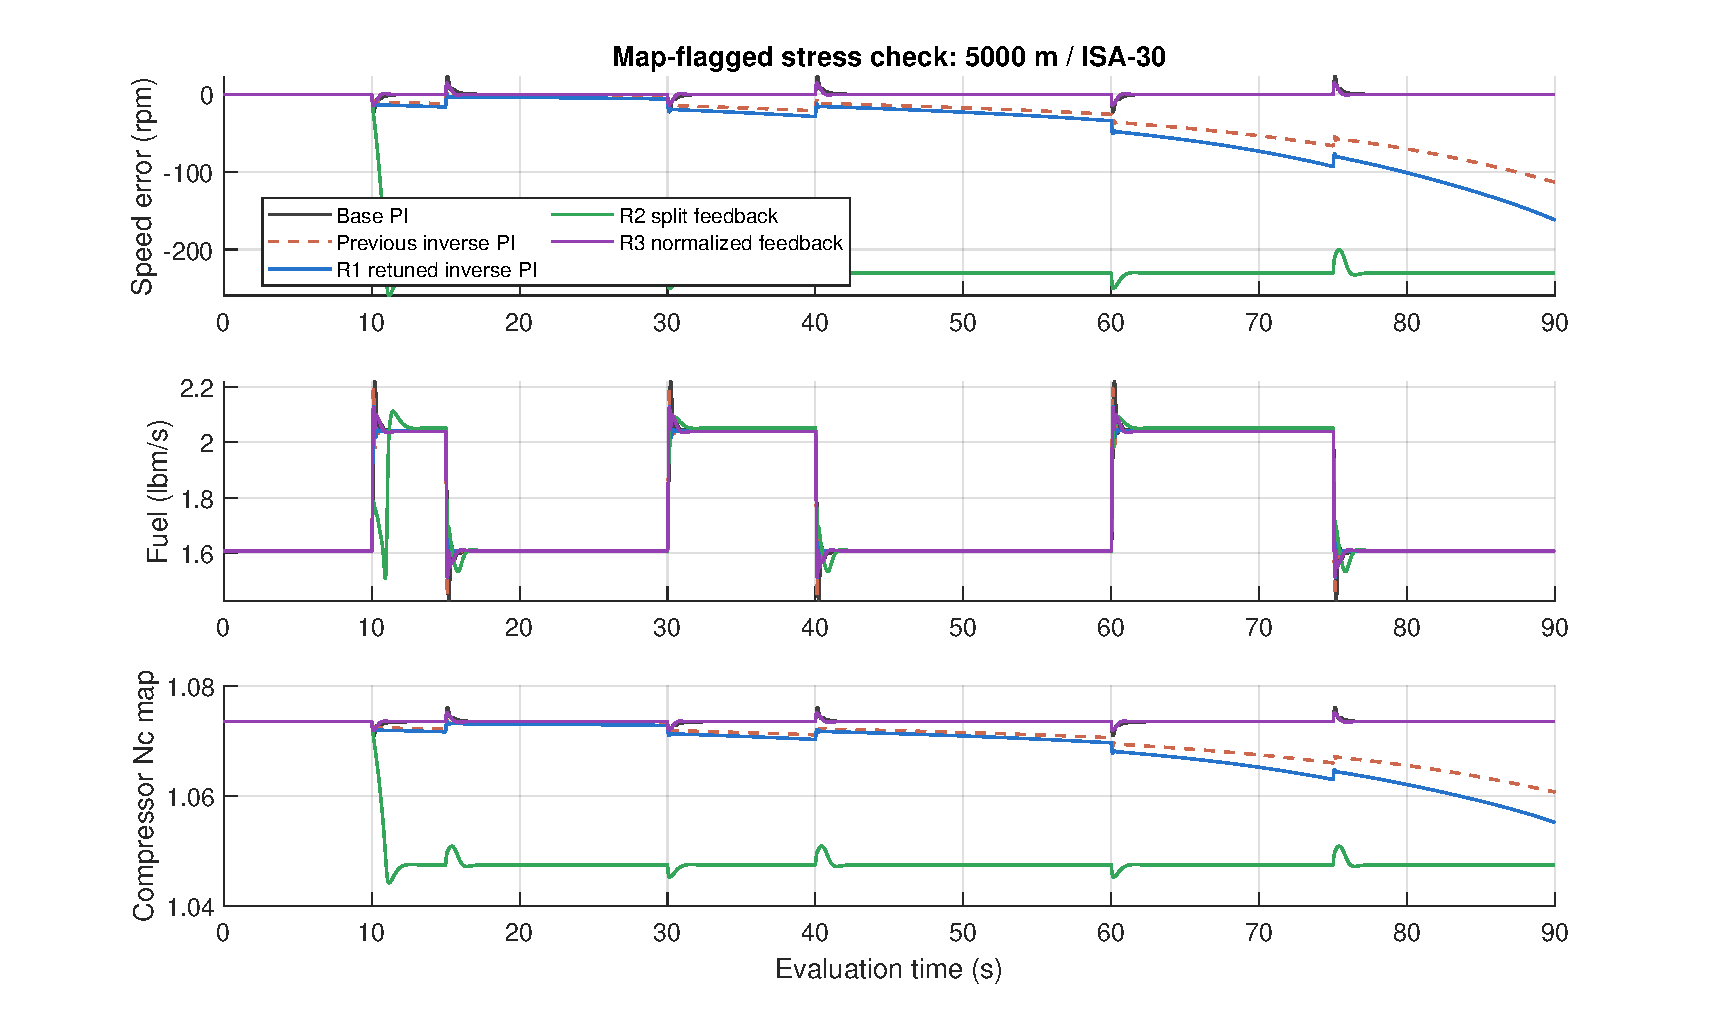
\includegraphics[width=\linewidth]{remedy_cold_case.pdf}\caption{The previously problematic 5000 m/ISA-30 case. The compressor-map limitation remains; controller guards do not validate the missing physical map range.}\end{figure}

This case distinguishes a gain adjustment from a structural safeguard. Lower gains do not change the sign of a faulty inverse error slope. R2 removes acceleration from integration but still integrates a static GP error. R3 explicitly substitutes speed feedback when its slope/map checks fail. Any improved numerical tracking here remains a result of the supplied boundary-clamped simulator; it is not evidence that the real engine is safe or accurately represented beyond the compressor map.

\section{Implementation and reproducibility}
The new study is saved under \path{results/gpr_remedies_20260914_220633}. The original inverse GPR and controller files are preserved. Three ready-to-run models are provided: \path{GasTurbine_Remedy1.mdl}, \path{GasTurbine_Remedy2.mdl} and \path{GasTurbine_Remedy3.mdl}. Their setup calls \path{tmats_gpr_remedy_setup.m}, which loads the frozen selected parameters and the same environmental GP.

The implementation is in \path{tmats_gpr_remedy_sfun.m}. \path{tmats_gp_mean_gradient.m} evaluates the exact posterior mean and its analytic input derivatives without copying the offline covariance factor at each sample. The original eight virtual-fuel signals are retained, with five added diagnostics: integrator error, proportional/damping correction, two inverse slopes and fallback activation.

Saved trajectories are independently replayed to check the proportional/damping formula, command summation, fuel saturation and discrete conditional integration. Grid simulations launched with the invalid-state stop instrumentation terminate at the first failed plant convergence or surge-margin criterion; earlier completed invalid runs are also rejected. Acceptance additionally requires the complete 150 s simulation, so a short rejected prefix cannot earn a misleading favorable RMSE. This instrumentation is separate from the saved controller models.

\path{run_tmats_gpr_remedies.m} performs tuning and transfer; \path{select_tmats_gpr_remedies.m} applies the declared objective; \path{diagnose_tmats_inverse_feedback.m} validates derivative calculations. Candidate definitions, all native MAT/CSV trajectories, selected parameters and the complete comparison table accompany the implementation. The GP's original 200 held-out observations are not used to refit the model during this controller study.

The tests contain no measurement noise or additional actuator lag. The selected controller should therefore be evaluated with those effects and with changed load/reference profiles before broader use. The present result establishes measured simulation tradeoffs and exposes the mechanisms that a fuel-value regression score alone could not reveal.

\begin{thebibliography}{9}
\bibitem{pid} MathWorks, \emph{Discrete-Time Proportional-Integral-Derivative Controllers}, derivative filtering and discrete implementation. \url{https://www.mathworks.com/help/control/ug/discrete-time-proportional-integral-derivative-pid-controller.html}.
\bibitem{gp} C. E. Rasmussen and C. K. I. Williams, \emph{Gaussian Processes for Machine Learning}, Chapter 2, MIT Press, 2006. \url{https://gaussianprocess.org/gpml/chapters/RW2.pdf}.
\end{thebibliography}
\end{document}
